
\documentclass{article}

\title{Lab 4}
\author{George Onwubuya}
\usepackage{fancyvrb}
\usepackage{minted}
\usepackage{graphicx}

\begin{document}
\maketitle

\section{Output Files}
\subsection{Output File 1}
\VerbatimInput{./sgemm-tiled.sh.o544199}

\subsection{Output File 2}
\VerbatimInput{./sgemm-tiled.sh.o544333}

\section{Performance Analysis}
\subsection{Square Matrices (n x n)}

\begin{tabular}{ |p{2.5cm}||p{2cm}|p{2cm}|p{2cm}|p{2cm}|p{2cm}|  }
 \hline
 \multicolumn{6}{|c|}{Execution Time (seconds) for Each Process } \\
 \hline
 Elements(nxn) & Setting Up & DeviceVar & Kernel & HostToDevice & DeviceToHost\\
 \hline
 1000 & 0.021003 & 0.173379 & 0.008233 & 0.004189 & 0.004426\\
 \hline
 2000 & 0.081349 & 0.182460 & 0.060868 & 0.017313 & 0.012964\\
 \hline
 4000 & 0.321950 & 0.186792 & 0.485511 & 0.068122 & 0.045862\\
 \hline
 8000 & 1.289725  & 0.184046 & 3.888804 & 0.274219 & 0.182651\\
  \hline
  \end{tabular}
  \\
  \\
  \\
  \subsection{Rectangle Matrices (A = m x k and B = k x n)} 
  \setlength{\parindent}{1cm}
  \begin{tabular}{ |p{2.5cm}||p{2cm}|p{2cm}|p{2cm}|p{2cm}|p{2cm}|  }
 \hline
 \multicolumn{6}{|c|}{Execution Time (seconds) for Each Process } \\
 \hline
 Elements (m,k,n) & Setting Up & DeviceVar & Kernel & HostToDevice & DeviceToHost\\
 \hline
 1000, 500, 500 & 0.009253 & 0.205076 & 0.002227 & 0.001798 & 0.002273\\
 \hline
 2000, 1000, 1000 & 0.031236 & 0.186218  & 0.016270 & 0.006258 & 0.007320\\
 \hline
 4000, 2000, 2000 & 0.119207 & 0.187957 & 0.121746 & 0.024576 & 0.022181\\
 \hline
 8000, 4000, 4000 & 0.481023  & 0.186625 & 0.971854 & 0.102642 & 0.098304 \\
  \hline
 \end{tabular}
 
 \subsection{Square Matrix Comparison BetweenTiled vs Non-Tiled}
 \setlength{\parindent}{1cm}
 \begin{tabular}{|p{3cm}||p{3cm}|p{3cm}|}
 \hline
 \multicolumn{3}{|c|}{Kernel Execution Times (seconds)}\\
 \hline
 Elements (n x n) & Tiled & Non-Tiled\\
 \hline
 1000 & 0.008233 & 0.022178\\
 \hline
 2000 & 0.060868 & 0.163624\\
 \hline
 4000 & 0.485511 & 1.308468\\
 \hline
 8000 & 3.888804 & 10.493221\\
 \hline
 \end{tabular}
 
\subsection{Tiled vs Non-Tiled Graphical Representation}
\graphicspath{./Picture1.png}
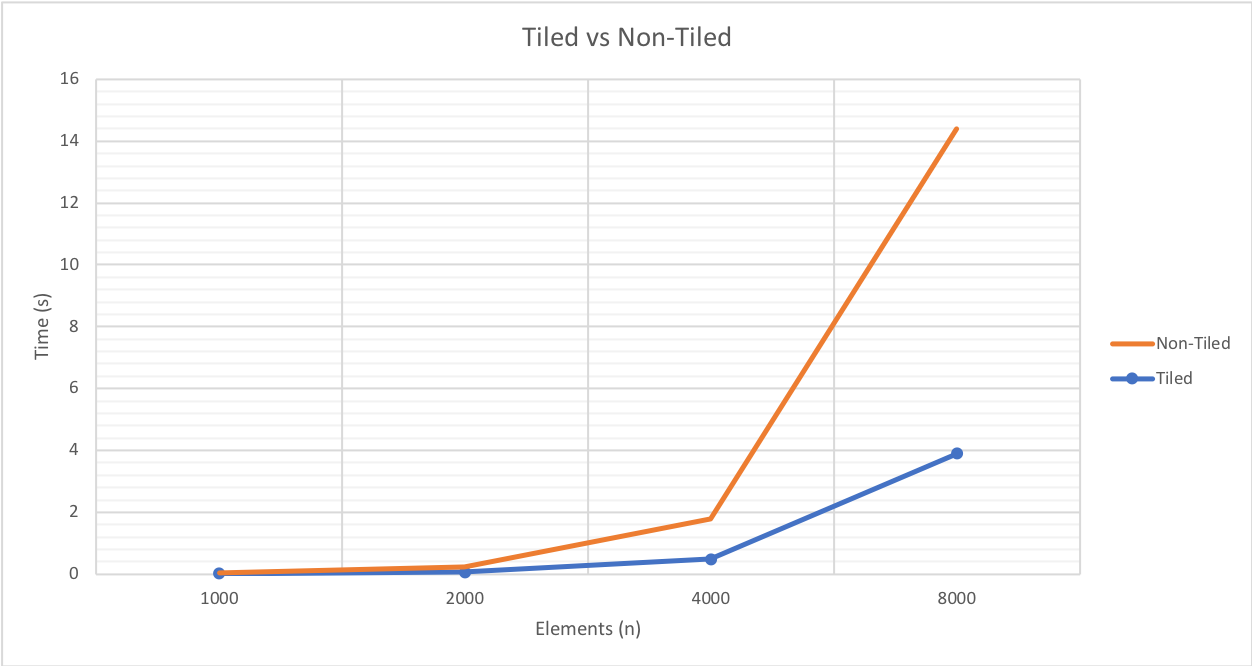
\includegraphics[width=\textwidth]{Picture1}
 
\subsection{Comments}
For the square matrices each process time followed a similar pattern except for the process of allocating of 'device variables'. The time taken to allocate device variables is approximately the same regardless of the number of elements.  As the number of elements increase the time taken setting up the problem, launching the kernel, copying data from the host to the device and vice versa also increases. There is an observable direct proportional relationship  between these processes and the number of elements. The same conclusion can be made for the rectangular matrices. 

\setlength{\parindent}{0cm}
\setlength{\parskip}{1em} 
There is an exponential increase in the kernel execution times associated with the tiled and non-tiled. However the non-tiled line graph shows a sharp increase in kernel execution time as the number of elements increase. This can be seen by the large spike between 4000 and 8000 elements on the graph. The tiled line graph does not exhibit that spike, as the purpose of tiling is reduce the number of global memory accesses. The graph shows that tiling reduces the kernel execution time by approximately a factor of 2.7.

\section{Answers}
\subsection{C(i)}   
The execution of nvcc --ptxas-options="-v" kernel.cu revealed resource usage statistics which include 25 registers/thread, 2K (2048 bytes) of shared memory, 360 bytes of constant memory[0] and 4 bytes of constant memory[2]. There are obvious limits to the number of threads allocated to a single streaming processor as defined by hardware specifications. For the GeForce GTX 280 GPU that has a compute capability of 1.3 these specifications include: 512 threads/block, 16K shared memory/multiprocessor, 16K registers/multiprocessor, 8 blocks/multiprocessor, 1024 threads/multiprocessor and 124 registers/thread. 

\setlength{\parindent}{0cm}
\setlength{\parskip}{1em} 
For this case, the block size is 16 x 16 = 256 threads and therefore the number of blocks/multiprocessor would be 1024/ 256 = 4. However, (256 threads x 25 reg/thread x 4 blocks/multiprocessor) $>$ 16K registers/multiprocessor. The number of registers per multiprocessor is a limiting factor and therefore only 2 blocks can run on a single microprocessor which would yield (256 x 2 x 25) $<$ 16K and hence the total number of threads that can be simultaneously scheduled for 30 single multiprocessors would be 256 x 2 x 30 = 15360. 

\section{Main}
\inputminted[breaklines, linenos]{c}{./main.cu}

\section{Kernel}
\inputminted[breaklines, linenos]{c}{./kernel.cu}

\end{document}




